\section{Deep learning}
\label{sec:nn}

In this manuscript, we adopt the point of view that a neural network is first a mathematical function, even though it derives its name from biological inspiration. That is, we won't discuss whether any of our works are biologically plausible or not, but we may provide biological interpretation when it happens.

In this section, we present a mathematical formalization and its biological interpretation. Then, we review a few important advances in the field before we finally present the most commonly used layers.

\subsection{Neural networks}
\label{sec:form}

A feed-forward neural network could originally be formalized as a composite function chaining linear and non-linear functions \citep{rumelhart1985learning,lecun1989backpropagation,lecun1995convolutional}. That whas still the case in 2012 when important breakthroughs regenerated a surge of interest in the field \citep{hinton2012deep,krizhevsky2012imagenet,simonyan2014very}. However, in more recent years, more complex architectures have emerged \citep{szegedy2015going,he2016deep,zoph2016neural,huang2017densely}, such that the former formalization does not suffice. We provide a definition for the first kind of neural networks (\defref{def:nn}) and use it to present its related concepts. Then we give a more generic definition (\defref{def:nn2}).

Note that in this manuscript, we only consider neural networks that are \emph{feed-forward} \citep{zell1994simulation, wiki:fnn}, as opposed to \emph{recurrent}.

We denote by $I_f$ the \textit{domain of definition} of a function $f$ ("I" stands for "input") and by $O_f = f(I_f)$ its \textit{image} ("O" stands for "output"), and we represent it as $I_f~\xrightarrow{f}~O_f$ or $f: I_f \to O_f$.

%\paragraph{Simple formalization}
\begin{definition}\textbf{Neural network (simply connected)}\\
Let $f$ be a function such that $I_f$ and $O_f$ are vector or tensor spaces.\\
$f$ is a \emph{(simply connected) neural network function} if there are a series of affine functions $(g_k)_{k=1,2,..,L}$ and a series of non-linear derivable univariate functions $(h_k)_{k=1,2,..,L}$ such that:
\begin{gather*}
\left\{
  \begin{array}{l}
    \forall k \in \llbracket 1, L \rrbracket, f_k = h_k \circ g_k, \\
    I_f = I_{f_1} \xrightarrow{f_1} O_{f_1} \cong I_{f_2} \xrightarrow{f_2} \dots \xrightarrow{f_L} O_{f_L} = O_f, \\
    f = f_{L} \circ ... \circ f_{2} \circ f_1
  \end{array}
\right.
\end{gather*}
The couple $(g_k, h_k)$ is called the \emph{$k$-th layer} of the neural network. $L$ is its depth.
For $x \in I_f$, we denote by $x_k = f_k \circ ... \circ f_{2} \circ f_1 (x)$ the \emph{activations} of the $k$-th layer. We denote by $\cn$ the set of neural network functions.
\label{def:nn}
\end{definition}

\begin{definition}\textbf{Activation function}\\
An \emph{activation function} $h$ is a real-valued univariate function that is non-linear and derivable, that is also defined by extension with the functional notation $h(v)[i] = h(v[i])$.
\end{definition}

\begin{definition}\textbf{Layer}\\
A layer is a couple $\cl = (g,h) : I \to O$, where $g : I \to O$ is a linear function, and $h: O \to O$ is an activation function. It computes the function
$$
y = h(g(x) + b)
$$
where $b$ is a constant called \emph{bias}.
\end{definition}

That is, in the simple formalization, a neural network is just a sequence of layers.

\begin{remark}The bias augments the expressivity of the layers. For notational convenience, we may sometimes omit to write it down.
\end{remark}

The most common activation function is the \emph{rectified linear unit} (ReLU)~\citep{glorot2011deep}, used for its better practical performances and faster computation times. It implements the \emph{rectifier} function $h: x \mapsto max(0,x)$ (with convention $h'(0) = 0$), as depicted on \figref{fig:relu}.

 \begin{figure}[htbp]
 \centering
 \begin{tikzpicture}
    \begin{axis}[
        domain=-3:5,
        ]
        \addplot+[mark=none,red,domain=-3:0] {0};
        \addplot+[mark=none,red,domain=0:5] {x};
    \end{axis}
 \end{tikzpicture}
 \caption{ReLU activation function}
 \label{fig:relu}
 \end{figure}

\paragraph{Examples}
Let $f: x \to y$ be a neural network. For example, if~$f$ is used to classify its input~$x$ in one of~$c$ classes, then its output~$y$ would be a vector of dimension~$c$,  and each dimension corresponds to a class. The prediction of~$f$ for the class of~$x$ is the dimension of~$y$ where it has the bigger value. Typically,~$f$ is terminated by a softmax activation~\citep{wiki:soft}, so that values of the output~$y$ fall in the range $[0,1]$, and so that~$y$ tends to have a dimension with a much bigger weight as to facilitates discrimination.

A neural network that comprises convolutional layers, \ie layers \st~$g$ is expressed with a convolution, is called a Convolutional Neural Network (CNN). A common example is the LeNet-5 architecture~\citep{lecun1989backpropagation} as depicted in \figref{fig:lenet}. It implements a function
$$
f = h_4 \circ g_4 \circ \cdots \circ h_1 \circ g_1
$$
where $g_1$ and $g_2$ are linear functions that applies 5x5 convolutions followed by subsampling, $h_1$, $h_2$ and $h_3$ are ReLU activations, and $h_4$ is a softmax activation. It was originally applied to the task of handwritten digit classifications (for example for automatically reading postal ZIP codes).

\begin{figure}[htp]
\centering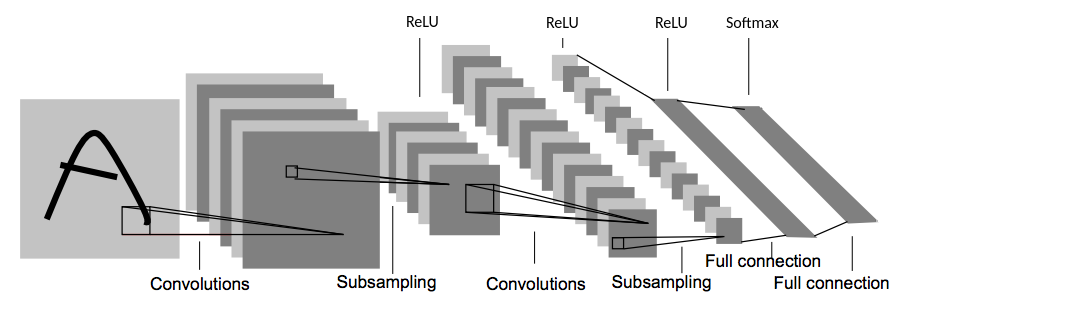
\includegraphics[scale=0.5]{chapter1/lenet5.png}
\caption{LeNet-5 \citep{lecun1989backpropagation}}
\label{fig:lenet}
\end{figure}

Another example is the VGG architecture, a very deep CNN, and was state-of-the-art in image classification in 2014 (\citeauthor{simonyan2014very}). It is depicted on \figref{fig:vgg}

\begin{figure}[htp]
\centering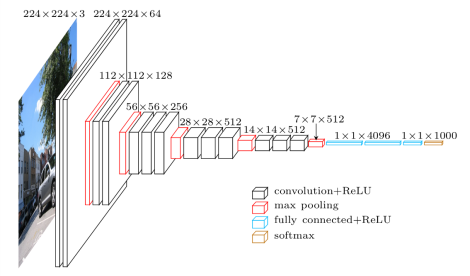
\includegraphics[scale=0.8]{chapter1/vgg16.png}
\caption{VGG-16 (\cite{simonyan2014very}, figure from~\cite{vgg})}
\label{fig:vgg}
\end{figure}

In more recent years, state-of-the-art architectures can no longer be described with a simple formalization.

%\paragraph{Generic formalization}
The former neural networks are said to be \emph{simply connected} because each layer only takes as input the output of the previous one. We'll give a more general definition after first defining branching operations.

\begin{definition}\textbf{Branching}\\
A \emph{binary branching operation} between two tensors, $x_{k_1} \Join x_{k_2}$, outputs, subject to shape compatibility, either their addition, either their concatenation along a rank, or their concatenation as a list.

A \emph{branching operation} between $n$ tensors, $x_{k_1} \Join x_{k_2} \Join \cdots \Join x_{k_n}$, is a composition of binary branching operations, or is the identity function $\id$ if $n = 1$.

Branching operations are also naturally defined on tensor-valued functions.% via their realizations.
\end{definition}

\begin{definition}\textbf{Neural network (generic definition)}\\
The set of \emph{neural network} functions $\cn$ is defined inductively as follows
\begin{enumerate}
  \item $Id \in \cn$
  \item $f \in \cn \wedge (g,h) \text{ is a layer} \wedge O_f \subset I_g \Rightarrow h \circ g \circ f \in \cn$
  \item for all shape compatible branching operations:\\
  $\quad f_1, f_2, \ldots, f_n \in \cn \Rightarrow  f_1 \Join f_2 \Join \cdots \Join f_n \in \cn$
\end{enumerate}
\label{def:nn2}
\end{definition}

\paragraph{Examples}
The neural network proposed in \citep{szegedy2015going}, called \emph{Inception}, use depth-wise concatenation of feature maps. Residual networks (ResNets, \cite{he2016deep}) make use of \emph{residual connections}, also called \emph{skip connections}, \ie an activation that is used as input in a lower level is added to another activation at an upper level, as depicted on \figref{fig:resnet}. Densely connected networks (DenseNets, \cite{huang2017densely}) have their activations concatenated with all lower level activations. These neural networks had demonstrated state of the art performances on the imagenet classification challenge \citep{deng2009imagenet}, outperforming simply connected neural networks. For example, DenseNet is depicted on \figref{fig:densenet}.
\label{par:branching_ex}

\begin{figure}[htp]
\centering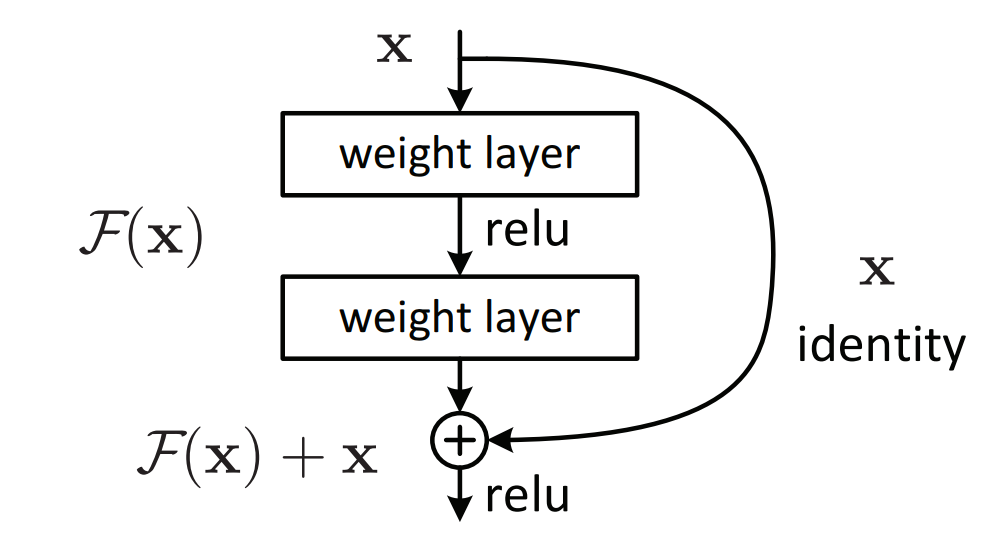
\includegraphics[scale=0.2]{chapter1/resnetmodule.png}
\caption{Module with a residual connection \citep{he2016deep}}
\label{fig:resnet}
\end{figure}

\begin{figure}[htp]
\centering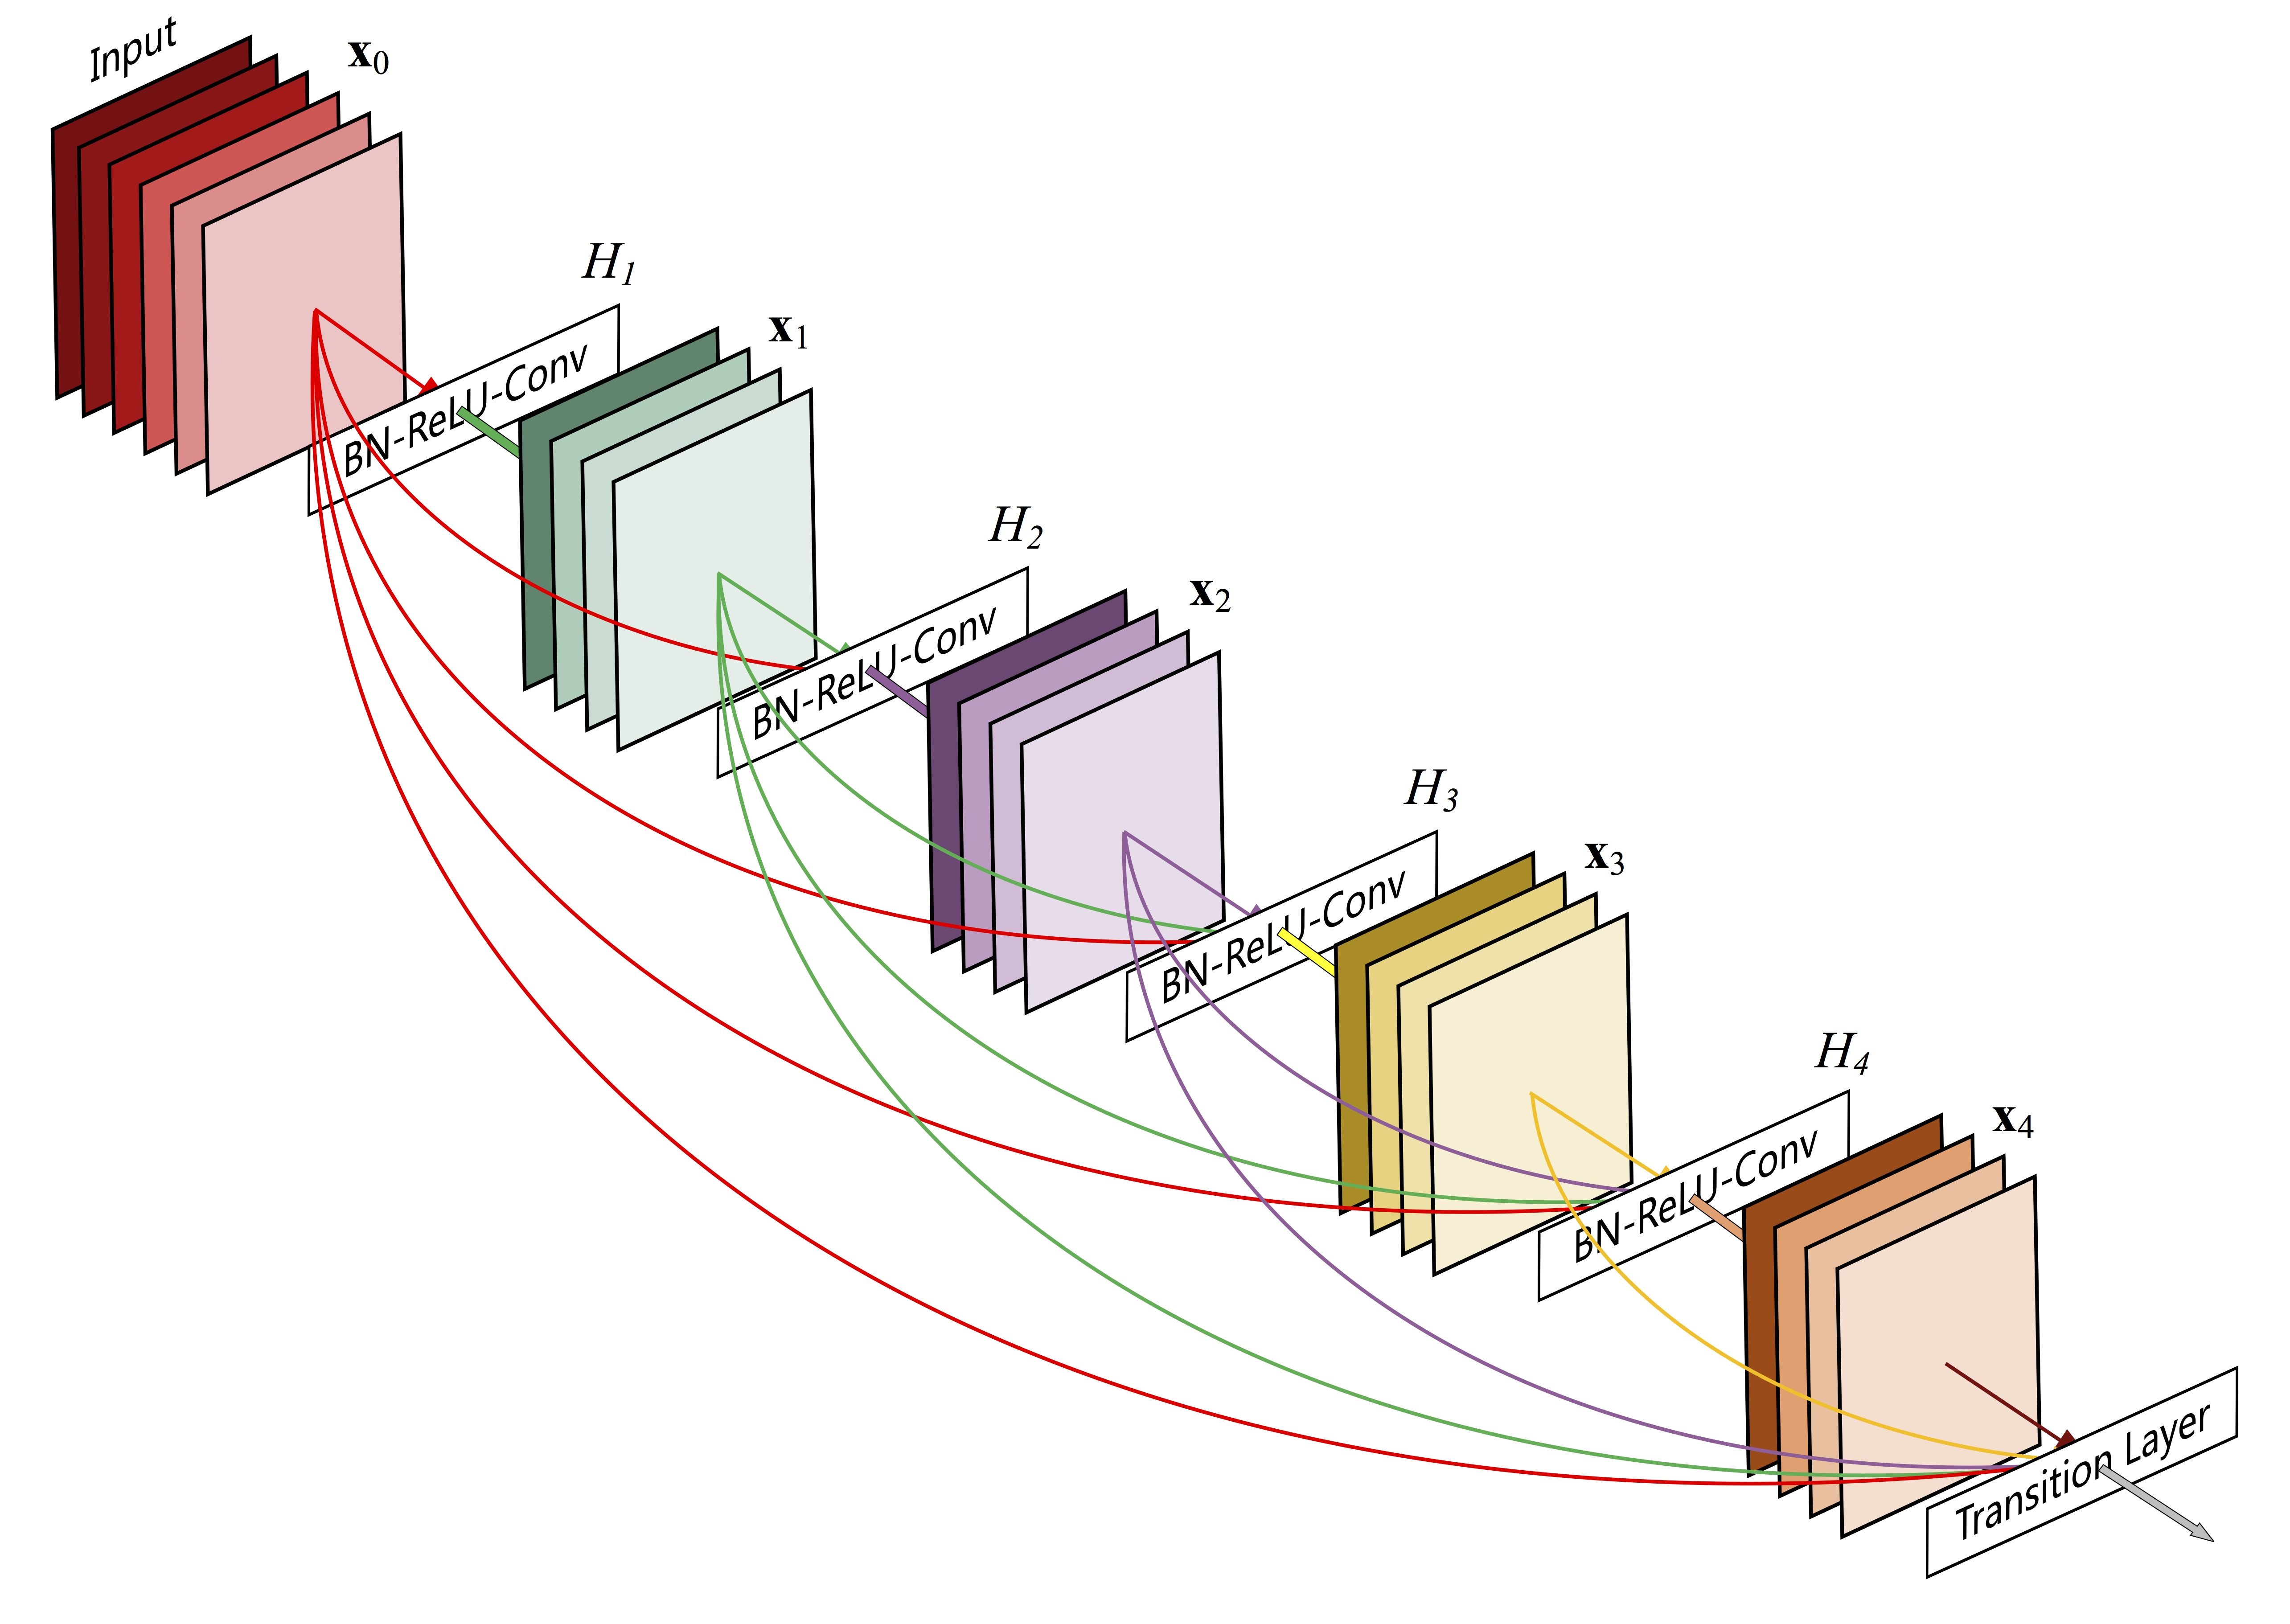
\includegraphics[scale=0.07]{chapter1/densenet.jpg}
\caption{DenseNet \citep{huang2017densely}}
\label{fig:densenet}
\end{figure}

\begin{remark}
For layer indexing convenience, we still use the simple formalization in the subsequent subsections, even though the presentation would be similar with the generic formalization.
\end{remark}

\subsection{Interpretation}
\label{sec:int}

Until now, we have formally introduced a neural network as a mathematical function. As its name suggests, such function can be indeed interpreted from a connectivity perspective \citep{lecun-87}.

\begin{definition}\textbf{Connectivity matrix}\\
Let $g$ a linear function. Without loss of generality subject to a flattening, let's suppose $I_g$ and $O_g$ are vector spaces. Then there exists a \emph{connectivity matrix}~$W_g$, such that:
\begin{gather*}
\forall x \in I_g, g(x) = W_g x
\end{gather*}
\end{definition}
We denote $W_k$ the connectivity matrix of the $k$-th layer.

\paragraph{Biological inspiration}
A \emph{neuron} is defined as a computational unit that is biologically inspired \citep{mcculloch1943logical}. Each neuron is capable of:
\begin{enumerate}[noitemsep,nolistsep]
\item receiving modulated signals from other neurons and aggregate them,
\item applying to the result an activation function,
\item passing the signal to other neurons.\\
\end{enumerate}
That is to say, each domain $\{I_{f_k}\}$ and $O_f$ can be interpreted as a layer of neurons, with one neuron for each dimension. The connectivity matrices $\{W_k\}$ describe the connections between each successive layers.
%The parameters of $\Theta_g$ are the modulation weights that characterize the connections.
A neuron is illustrated on \figref{fig:neuron}.

\begin{figure}[h!tb]
\centering
\begin{tikzpicture}[
init/.style={
  draw,
  circle,
  inner sep=2pt,
  font=\Huge,
  join = by o-latex
},
squa/.style={
  draw,
  inner sep=2pt,
  font=\Large,
  join = by -latex
},
start chain=2,node distance=13mm
]
\node[on chain=2] 
  (x2) {$x_2$};
%\node[on chain=2,join=by o-latex] 
%  {$w_2$};
\node[on chain=2,init] (sigma)
  {$\displaystyle\Sigma$};
\node[on chain=2,squa,label=above:{\parbox{2cm}{\centering activation}}]   
  {$h$};
\node[on chain=2,join=by -o] 
  {$y$};
\begin{scope}[start chain=1]
\node[on chain=1] at (0,1.5cm) 
  (x1) {$x_1$};
%\node[on chain=1,join=by o-latex] 
%  (w1) {$w_1$};
\end{scope}
\begin{scope}[start chain=3]
\node[on chain=3] at (0,-1.5cm) 
  (x3) {$x_3$};
%\node[on chain=3,label=below:Weights,join=by o-latex] 
%  (w3) {$w_3$};
\end{scope}
\node[label=above:{\centering bias}] at (sigma|-x1) (b) {};

\draw[o-latex] (x1) -- (sigma);
\draw[o-latex] (x3) -- (sigma);
\draw[o-latex] (b) -- (sigma);

\node at (1cm,1.2cm) {$w_1$};
\node at (1cm,0.2cm) {$w_2$};
\node at (1cm,-0.5cm) {$w_3$};
\node at (2.37cm,0.9cm) {$b$};

%\draw[decorate,decoration={brace,mirror}] (x1.north west) -- node[left=10pt] {Inputs} (x3.south west);
\end{tikzpicture}
\caption{A neuron}
\label{fig:neuron}
\end{figure}

\subsection{Training}
\label{sec:training}

Given an objective function $F$, training is the process of incrementally modifying a neural network $f$ upon obtaining a better approximation of $F$.
The most used training algorithms are based on gradient descent, as proposed in \citep{widrow1960adaptive}. These algorithms became popular since \citep{rumelhart1985learning}. Informally, $f$ is parameterized with initial weights that characterize its linear parts. These weights are modified step by step. At each step, a batch of samples are fed to the network, and their approximation errors sum to a loss. The weights of the network are updated in the opposite direction to their gradient with respect to that loss. If the samples are shuffled and grouped in batches, this is called \emph{Stochastic} gradient descent (SGD). Stochastic approximation \citep{robbins1985stochastic} tends to minimize effects of outliers on the training and is agnostic of the order in which the samples are fed.

%All possible realizations of $f$ through its weights draw a family $N$ which expressivity is crucial for the success of the training. The common points between $f$ and other objects of $N$ define what is called a neural network \emph{architecture}. That is

\begin{definition}\textbf{Weights}\\
Let consider the $k$-th layer of a neural network $f$. We define its weights as coordinates of a vector $\theta_k$, called the \emph{weight kernel}, such that:
\begin{gather*}
  \forall (i,j),
    \begin{cases}
      \exists p, W_k[i,j] := \theta_k[p] \\
      \text{ or } W_k[i,j] = 0
    \end{cases}
\end{gather*}
\end{definition}
A weight $p$ that appears multiple times in $W_k$ is said to be \emph{shared}. Two parameters of $W_k$ that share a same weight $p$ are said to be \emph{tied}. The number of weights of the $k$-th layer is $n_1^{(\theta_k)}$.

\paragraph{Learning}
A \emph{loss} function $\mathcal{L}$ penalizes the output $x_L = f(x)$ relatively to the approximation error $|f(x) - F(x)|$. Gradient w.r.t.~$\theta_k$, denoted $\vec{\bigtriangledown}_{\theta_k}$, is used to update the weights via an optimization algorithm based on gradient descent and a learning rate $\alpha$, that is:
\begin{gather}
\theta_k^{(\text{new})} = \theta_k^{(\text{old})} - \alpha \cdot \vec{\bigtriangledown}_{\theta_k} \left( \mathcal{L}\left( x_L, \theta_k^{(\text{old})} \right) + \ccr\left( \theta_k^{(\text{old})} \right) \right)
\end{gather}
where $\ccr$~is a regularizer, and where $\alpha$~can be a scalar or a vector and $\cdot$~can denote outer or coordinate-wise product, depending on the optimization algorithm that is used.

\paragraph{Linear complexity}
Without loss of generality, we assume that the neural network is simply connected. Thanks to the chain rule, $\vec{\bigtriangledown}_{\theta_k}$ can be computed using gradients that are w.r.t. $x_k$, denoted $\vec{\bigtriangledown}_{x_k}$, which in turn can be computed using gradients w.r.t. outputs of the next layer $k+1$, up to the gradients given on the output layer.

That is:
\begin{align}
  \vec{\bigtriangledown}_{\theta_k} & = J_{\theta_k}(x_k) \vec{\bigtriangledown}_{x_k} \\
  \begin{split}
  \vec{\bigtriangledown}_{x_k} & = J_{x_k}(x_{k+1}) \vec{\bigtriangledown}_{x_{k+1}} \\
  \vec{\bigtriangledown}_{x_{k+1}} & = J_{x_{k+1}}(x_{k+2}) \vec{\bigtriangledown}_{x_{k+2}} \\
  \quad \quad \ldots\\
  \vec{\bigtriangledown}_{x_{L-1}} & = J_{x_{L-1}}(x_{L}) \vec{\bigtriangledown}_{x_{L}}
  \label{eq:bp}
  \end{split}
\end{align}
Obtaining,
\begin{align}
  \vec{\bigtriangledown}_{\theta_k} = J_{\theta_k}(x_k) (\prod_{p=k}^{L-1} J_{x_p}(x_{p+1})) \vec{\bigtriangledown}_{x_L}
\end{align}
where $J_{\text{wrt}}(.)$ are the respective jacobians which can be determined with the layer's expressions and the $\{x_k\}$; and $\vec{\bigtriangledown}_{x_L}$ can be determined using $\mathcal{L}$, $\ccr$ and $x_L$.
This allows to compute the gradients with a complexity that is linear with the number of weights (only one computation of the activations), instead of being quadratic if it were done with the difference quotient expression of the derivatives (one more computation of the activations for each weight).

\paragraph{Backpropagation}
We can remark that \eqref{eq:bp} rewrites as
\begin{align}
  \begin{split}
  \vec{\bigtriangledown}_{x_k} & = J_{x_k}(x_{k+1}) \vec{\bigtriangledown}_{x_{k+1}} \\ 
                               & = J_{x'_k}(h(x'_k)) J_{x_k}(W_k x_k) \vec{\bigtriangledown}_{x_{k+1}}
  \end{split}
\end{align}
where $x'_k = W_k x_k$, and these jacobians can be expressed as:
\begin{align}
  \begin{split}
  J_{x'_k}(h(x'_k)) & [i,j] = \delta_i^j h'(x'_k[i])\\
  J_{x'_k}(h(x'_k)) & = I \hspace{2pt} h'(x'_k)
  \end{split}\\
  J_{x_k}(W_k x_k) & = W_k^T
\end{align}
That means that we can write $\vec{\bigtriangledown}_{x_k} = (\widetilde{h}_k \circ \widetilde{g}_k)(\vec{\bigtriangledown}_{x_{k+1}})$ such that the connectivity matrix $\widetilde{W}_k$ is obtained by transposition. This can be interpreted as gradient calculation being a \emph{back-propagation} on the same neural network, in opposition of the \emph{forward-propagation} done to compute the output.

\subsection{Some historical advances}
\label{sec:hist}

\paragraph{Universal approximation}
Early researches have shown that neural networks with one level of depth can approximate any real-valued function defined on a compact subset of~$\bbr^n$. This result was first proved for sigmoidal activations \citep{cybenko1989approximation}, and then it was shown it did not depend on the sigmoidal activations \citep{hornik1989multilayer,hornik1991approximation}.

For example, this result brings theoretical justification that objective functions exists (even though it does not inform whether an algorithm to approach it exists or is efficient).

\paragraph{Computational difficulty}
However, reaching such objective is a computationally difficult problem, which drove back interest from the field. Thanks to better hardware and to using better initialization schemes that speed up learning, researchers started to report more successes with deep neural networks \citep{hinton2006fast,glorot2010understanding} ; see \citep{bengio2009learning} for a review of this period. It ultimately came to a surge of interest in the field after a significant breakthrough on the imagenet dataset \citep{deng2009imagenet} with deep CNNs \citep{krizhevsky2012imagenet}. The use of the fast ReLU activation function \citep{glorot2011deep} as well as leveraging graphical processing units with CUDA \citep{nickolls2008scalable} were also key factors in overcoming this computational difficulty.

\paragraph{Adoption of ReLU activations}
Historically, sigmoidal and tanh activations were mostly used \citep{cybenko1989approximation, lecun1989backpropagation}. However in recent practice, the ReLU activation (first introduced as the \emph{positive part}, \cite{jarrett2009best}), become the most used activation, as it was demonstrated to be faster and to obtain better results \citep{glorot2011deep}. ReLU originated numerous variants \eg \emph{leaky rectified linear unit} \citep{maas2013rectifier}, \emph{parametric rectified linear unit} (PReLU, \cite{he2015delving}), \emph{exponential linear unit} (ELU, \cite{clevert2015fast}), \emph{scaled exponential linear unit} (SELU, \cite{Klambauer2017self}), each one having particular advantages in some applications.

\paragraph{Avoiding overfitting}
Neural networks, like any other machine learning technique, may overfit. That is, a model may behave well on the training set but fails to generalize well on unseen examples. The introduction of dropout \citep{srivastava2014dropout} have helped models with more parameters to be less prone to overfitting, as dropout consists in hiding some parts of the training samples and their intermediate activations. Another good practice is to normalize per batch \citep{ioffe2015batch}.
%Dropout consists in randomly setting a certain number of neurons to zero during the training phase (compensated at test time by scaling down the whole layer). The idea is that some part of the training samples are hidden to the model, so that it cannot overfit on them.

\paragraph{Expressivity and expressive efficiency}
The study of the \emph{expressivity} (also called \emph{representational power}) of families of neural networks is the field that is interested in the range of functions that can be realized or approximated by this family \citep{haastad1991power,pascanu2013number}. In general, given a maximal error~$\epsilon$ and an objective~$F$, the more expressive is a family $N \subset \cn$, the more likely it is to contain an approximation $f \in N$ such that $d(f,F) < \epsilon$. However, if we consider the approximation $f_{min} \in N$ that have the lowest number of neurons, it is possible that~$f_{min}$ is still too large and may be unpractical. For this reason, expressivity is often studied along the related notion of \emph{expressive efficiency} \citep{delalleau2011shallow,cohen2018boosting}.
\label{par:expr}

\paragraph{Rectifier neural netowrks}
Of particular interest for the intuition is a result stating that a simply connected neural networks with only ReLU activations (a rectifier neural network) is a piecewise linear function \citep{pascanu2013number,montufar2014number}, and that conversely any piecewise linear function is also a rectifier neural network such that an upper bound of its depth is logarithmically related to the input dimension (\cite{arora2018understanding}, th. 2.1.). Their expressive efficiency have also been demonstrated compared to neural networks using threshold or sigmoid activations~\citep{pan2016expressiveness}.

\paragraph{Benefits of depth}
Expressive efficiency analysis have demonstrated the benefits of depth, \ie a shallow neural network would need an unfeasible large number of neurons to approximate the function of a deep neural network (\eg \cite{delalleau2011shallow,bianchini2014complexity,poggio2015theory,eldan2016power,poole2016exponential,raghu2016expressive,cohen2016convolutional,mhaskar2016learning,lin2017does,arora2018understanding}). This field seeks to give theoretical grounds to the practical observation that state-of-the-art architectures are getting deeper. 

\paragraph{Benefits of branching operations}
Recent works have provided rationales supporting benefits of using branching operations, thus giving justifications for architectures obtained with the generic formalization. In particular, \citep{cohen2018boosting} have analyzed the impact of residual connections used in Wavenet-like architectures \citep{van2016wavenet} in terms of expressive efficiency, using tools from the field of tensor analysis ; \citep{orhan2018skip} have empirically demonstrated that skip connections can resolve some inefficiency problems inherent of fully-connected networks (dead activations, activations that are always equal, linearly dependent sets of activations).


\subsection{Common layers}
\label{sec:layer}

\begin{definition}\textbf{Connections}\\
The set of \emph{connections} of a layer $(g,h)$, denoted $C_g$, is defined as:
\begin{gather*}
  C_g = \{(i,j), \exists p, W_g[i,j] := \theta_g[p]\}
\end{gather*}
We have $0 \leq |C_g| \leq n_1^{(W_g)} n_2^{(W_g)}$.
\end{definition}

\begin{definition}\textbf{Dense layer}\\
A \emph{dense layer} $(g,h)$ is a layer such that $|C_g| = n_1^{(W_g)} n_2^{(W_g)}$, \ie all possible connections exist. The map $(i,j) \mapsto p$ is usually a bijection, meaning that there is no weight sharing.
\end{definition}

A neural network made only of dense layers is called a Multi-Layer Perceptron (MLP, \cite{hornik1989multilayer}).

\begin{definition}\textbf{Partially connected layer}\\{}
A \emph{partially connected layer} $(g,h)$ is a layer such that $|C_g| < n_1^{(W_g)} n_2^{(W_g)}$.

A \emph{sparsely connected layer} $(g,h)$ is a layer such that $|C_g| \ll n_1^{(W_g)} n_2^{(W_g)}$.
\end{definition}

\begin{definition}\textbf{Convolutional layer}\\
A \emph{$n$-dimensional convolutional layer} $(g,h)$ is such that the weight kernel~$\theta_g$ can be reshaped into a tensor $w$ of rank $n+2$, and such that
\begin{gather*}
\left\{
\begin{array}{l}
  I_g \mbox{ and } O_g \mbox{ are tensor spaces of rank }n+1 \\
  \forall x \in I_g, g(x) = (g(x)_q = \sum\limits_p{x_p \ast^n w_{p,q}})_{\forall q}
\end{array}
\right.
\end{gather*}
where $p$ and $q$ index slices along the last ranks.
\label{def:convlayer}
\end{definition}

A neural network that contains convolutional layers is called convolutional neural network (CNN).

\begin{definition}\textbf{Feature maps and input channels}\\
The slices $g(x)_q$ are typically called \textit{feature maps}, and the slices $x_p$ are called \textit{input channels}. Let's denote by $n_o = n_{n+1}^{(O_g)}$ and $n_i =n_{n+1}^{(I_g)}$ the number of feature maps and input channels.
In other words, \defref{def:convlayer} means that for each feature maps, a convolution layer computes $n_i$ convolutions and sums them, computing a total if $n_i \times n_o$ convolutions.
\end{definition}

\begin{remark}
Note that because they are simply summed, entries of two different input channels that have the same coordinates are assumed to share some sort of relationship. For instance on images, entries of each input channel (typically corresponding to Red, Green and Blue channels) that have the same coordinates share the same pixel location.
\end{remark}

\paragraph{Benefits of convolutional layers}
Comparatively with dense layers, convolution layers enjoy a significant decrease in the number of weights. For example, an input $2 \times 2$ convolution on images with $3$-color input channels, would breed only $12$ weights per feature maps, independently of the numbers of input neurons. On image datasets, their usage also breeds a significant boost in performance compared with dense layers~\citep{krizhevsky2012imagenet}, for they allow to take advantage of the topology of the inputs while dense layers do not~\citep{lecun1995convolutional}. A more thorough comparison and explanation of their assets will be discussed in \secref{sec:cnnvsmlp}.

\paragraph{Decrease of spatial dimensions}
Given a tensor input $x$, the $n$-dimensional convolutions between the inputs channels $x_p$ and slices of a weight tensor $w_{p,q}$ would result in outputs $y_q$ of shape $n_1^{(x)} - n_1^{(w)} + 1 \times \ldots \times n_n^{(x)} - n_n^{(w)} + 1$. So, in order to preserve shapes, a padding operation must pad $x$ with $n_1^{(w)} - 1 \times \ldots \times n_n^{(w)} - 1$ zeros beforehand. For example, the padding function of the library \emph{tensorflow}~\citep{tensorflow2015-whitepaper} pads each rank with a balanced number of zeros on the left and right indices (except if $n_t^{(w)} - 1$ is odd then there is one more zero on the left).

\begin{definition}\textbf{Padding}\\
A convolutional layer with \emph{padding} $(g, h)$ is such that $g$ can be decomposed as $g = g_\text{pad} \circ g'$, where $g'$ is the linear part of a convolution layer as in \defref{def:convlayer}, and $g_\text{pad}$ is an operation that pads zeros to its inputs such that $g$ preserves tensor shapes.
\end{definition}

\begin{remark}
One asset of padding operations is that they limit the possible loss of information on the borders of the subsequent convolutions, as well as preventing a decrease in size. Moreover, preserving shape is needed to build some neural network architectures, especially for ones with branching operations \eg examples in \secref{par:branching_ex}. On the other hand, they increase memory and computational footprints.
\end{remark}

\begin{definition}\textbf{Stride}\\
A convolutional layer with \emph{stride} is a convolutional layer that computes strided convolutions (with stride $> 1$) instead of convolutions.
\end{definition}

\begin{definition}\textbf{Pooling}\\
A layer with \textit{pooling} $(g,h)$ is such that $g$ can be decomposed as $g = g' \circ g_\text{pool}$, where $g_\text{pool}$ is a pooling operation.
\end{definition}

Layers with stride or pooling downscale the signals that passes through the layer. These types of layers allows to compute features at a coarser level, giving the intuition that the deeper a layer is in the network, the more abstract is the information captured by the weights of the layer. Additional, from a practical point of view, they contribute to lower the computational complexity at deeper levels.

\paragraph{A simple result}
In two dimensions, convolutional operations can be rewritten as a matrix-vector multiplication where the matrix is Toeplitz. We show below that it is still the case in $n$~dimensions.

\begin{proposition}\textbf{Connectivity matrix of a convolution with padding}\\
A convolutional layer with padding $(g, h)$ is equivalently defined as its connectivity matrix $W_g$ being a $n_i \times n_o$ block matrix such that its blocks are Toeplitz matrices, and where each block corresponds to a couple $(p,q)$ of input channel~$p$ and feature map~$q$.
\end{proposition}

\begin{proof}
Let's consider the slices indexed by $p$ and $q$, and to simplify the notations, let's drop the subscripts $\hspace{0pt}_{p,q}$. We recall from \defref{def:convdef} that
\begin{align*}
  y &= (x \ast^n w)[j_1, \ldots, j_n] \\
 &= \displaystyle \sum_{k_1=1}^{n_1^{(w)}} \cdots \sum_{k_n=1}^{n_n^{(w)}}
    x[j_1 + n_1^{(w)} - k_1, \ldots, j_n + n_n^{(w)} - k_n] \hspace{2pt} w[k_1, \ldots, k_n] \\
 &= \displaystyle \sum_{i_1=j_1}^{j_1 + n_1^{(w)} - 1} \cdots \sum_{i_n=j_n}^{j_n + n_n^{(w)} - 1}
    x[i_1, \ldots, i_n] \hspace{2pt} w[j_1 + n_1^{(w)} - i_1, \ldots, j_n + n_n^{(w)} - i_n] \\
 &= \displaystyle \sum_{i_1=1}^{n_1^{(x)}} \cdots \sum_{i_n=1}^{n_n^{(x)}}
    x[i_1, \ldots, i_n] \hspace{2pt} \widetilde{w}[i_1, j_1, \ldots, i_n, j_n] \\
 & \text{ where } \widetilde{w}[i_1, j_1, \ldots, i_n, j_n] = \\
 & \quad \quad
 \begin{cases}
   w[j_1 + n_1^{(w)} - i_1, \ldots, j_n + n_n^{(w)} - i_n] & \text{if } \forall t, 0 \le i_t - j_t \le n_t^{(w)} - 1 \\
   0 & \text{otherwise}
 \end{cases}
\end{align*}
Using Einstein summation convention as in~\eqref{eq:indices} and permuting indices, we recognize the following tensor contraction
\begin{align}
y_{j_1 \cdots j_n} = x_{i_1 \cdots i_n} \widetilde{w} \hspace{1pt}^{i_1 \cdots i_n} \hspace{0pt}_{j_1 \cdots j_n} \label{eq:toep1}
\end{align}
Following \propref{prop:matprodeq}, we reshape~\eqref{eq:toep1} as a matrix product. To reshape $y \mapsto Y$, we use the row major order bijections $g_j$ as in~\eqref{eq:rowmajor} defined onto $\{(j_1, \ldots, j_n), \forall t, 1 \le j_t \le n_t^{(y)}\}$. To reshape $x \mapsto X$, we use the same row major order bijection $g_j$, however defined on the indices that support non zero-padded values, so that zero-padded values are lost after reshaping. That is, we use a bijection $g_i$ such that $g_i(i_1, i_2, \ldots, i_n) = g_j(i_1 - o_1, i_2 - o_2, \ldots, i_n - o_n)$ defined if and only if $\forall t, 1 + o_t \le i_t \le n_t^{(y)}$, where the $\{o_t\}$ are the starting offsets of the non zero-padded values. $\widetilde{w} \mapsto W$ is reshaped by using $g_j$ for its covariant indices, and $g_i$ for its contravariant indices. The entries lost by using $g_i$ do not matter because they would have been nullified by the resulting matrix product. We remark that $W$ is exactly the block $(p,q)$ of $W_g$ (and not of $W_{g'}$). Now let's prove that it is a Toeplitz matrix.

Thanks to the linearity of the expression~\eqref{eq:rowmajor} of $g_j$, by denoting $i'_t = i_t - o_t$, we obtain
\begin{gather}
  g_i(i_1, i_2, \ldots, i_n) - g_j(j_1, j_2, \ldots, j_n) = g_j(i'_1 - j_1, i'_2 - j_2, \ldots, i'_n - j_n)
\label{eq:toep2}
\end{gather}

To simplify the notations, let's drop the arguments of $g_i$ and $g_j$. By bijectivity of $g_j$, \eqref{eq:toep2} tells us that $g_i - g_j$ remains constant if and only if $i'_t - j_t$ remains constant for all $t$. Recall that 
\begin{gather}
  W[g_i,g_j] =
 \begin{cases}
   w[j_1 + n_1^{(w)} - i'_1, \ldots, j_n + n_n^{(w)} - i'_n] & \text{if } \forall t, 0 \le i'_t - j_t \le n_t^{(w)} - 1 \\
   0 & \text{otherwise}
 \end{cases}
\label{eq:toep3}
\end{gather}
Hence, on a diagonal of $W$, $g_i - g_j$ remaining constant means that $W[g_i,g_j]$ also remains constants. So $W$ is a Toeplitz matrix.

The converse is also true as we used invertible functions in the index spaces through the proof.
\end{proof}

\begin{remark}
Note that the proof does not hold in case there is no padding. This is due to border effects when the index of the $n$\powth rank resets in the definition of the row-major ordering function $g_j$ that would be used. Indeed, under appropriate definitions, the matrices could be seen as almost Toeplitz.
\end{remark}

This proposition provides an equivalent-characterization of convolutional layers by their connectivity matrix. Therefore, a first avenue to define convolutions on graph signals could be to define them with the connectivity matrix being as in this characterization. However, the Toeplitz property implies that the dimensions have a specific order, which is not possible when dimensions correspond to vertices of a graph. This is because permuting the order of the vertices wouldn't change the graph, but would change the connectivity matrix (which cannot be Toeplitz for every ordering).

%\subsection{Examples of regularization}

% \paragraph{Overfitting}
% \todo{}

% A layer with \textit{dropout} $(g,h)$ is such that $h = h_1 \circ h_2$, where $(g,h_2)$ is a layer and $h_1$ is a dropout operation~\citep{srivastava2014dropout}. When dropout is used, a certain number of neurons are randomly set to zero during the training phase, compensated at test time by scaling down the whole layer. This is done to prevent overfitting.

% \subsection{Examples of architecture}
% \label{sec:nn_arch}

% \todo{rephrase}

% A multilayer perceptron (MLP)~\citep{hornik1989multilayer} is a neural network composed of only dense layers.
% A convolutional neural network (CNN)~\citep{lecun1998gradient} is a neural network composed of convolutional layers.

% Neural networks are commonly used for machine learning tasks. For example, to perform supervised classification, we usually add a dense output layer $s=(g_{L+1},h_{L+1})$ with as many neurons as classes. We measure the error between an output and its expected output with a discriminative loss function $\mathcal{L}$. During the training phase, the weights of the network are adapted for the classification task based on the errors that are back-propagated~\citep{hornik1989multilayer} via the chain rule and according to a chosen optimization algorithm (\eg \cite{bottou2010large}).
